
\section{Pascal GP100 Whitepaper}
The Tesla P100 has 5.3TFLOPS of FP64 performance, double as much (10.6 TFLOPS) of FP32, and four times as much (21.2 TFLOPS) of FP16.
The 16-bit floating point precision ability is though for Deep Learning.
Deep Learning does not require higher precision and this brings both higher speed and higher available storage for bigger models.

\subsection{Microprocessor architecture}
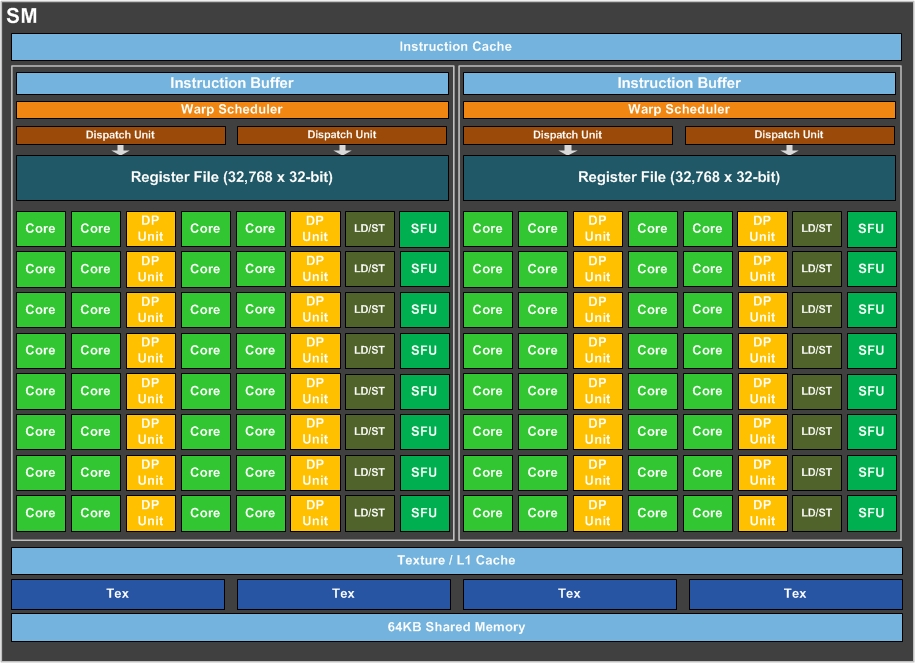
\includegraphics[width=0.9\linewidth]{gp100_sm}
\subsubsection{Processor structure}
It is composed of an array of GPCs, formed by TPCs, consisting of 2 SMs with 64 CUDA FP32 Cores and 4 texture units each.
The GP100 processor has 6 GPCs with 10 SMs each.
This makes a total of 3840 CUDA Cores
4 of the SMs on the chip are turned off, giving a total of 56 available SM units.

Each SM has 32 FP32 CUDA Cores, an instruction buffer, and a warp scheduler with two dispatch units.
Since the register file size per CUDA Core is doubled, there can be more thread blocks running concurrently.

The scheduler data path is changed with respect to Kepler and Maxwell.
A big improvement in the scheduler in comparison to Maxwell is that each warp scheduler can dispatch two warp instructions per clock.
This allows up to \textbf{TODO: What does UP TO mean?} twice FP16 throughput vs FP32.
There is also a 2:1 ratio of FP64 to FP32 CUDA Cores per SM, which now works better with the data path.
\subsubsection{Memory hierarchy}
Same as before

\subsubsection{On-chip memory}
The L1/shared memory structure has not changed since Maxwell.
Each SM has 64KB of shared memory (up to 32KB per Thread Block), with an additional L1/texture cache.
This improves on the 64KB configurable shared memory/L1 cache of Fermi and Kepler.

There are eight 512-bit memory controllers to communicate with off-chip memory.
There is a unifed 4096KB L2 cache, which gives 512KB per memory controller.

\subsubsection{Off-chip memory HBM2}
Each stack of HBM2 is controlled by a pair of memory controllers.
Stacked memory uses less surface, which allows denser servers.
A HBM2 stack is composed by 4 or 8 dies with microscopic wires which go down the stack.
Each HBM2 die has a 8Gb capacity, giving a total of 4 or 8GB per stack.
The stacks have to be connected to the chip via a passive silicon interposer.
The height of the dies is adjusted (the top die is thicker) in order to make good contact with the heat sink.
HBM1 supported only 4 dies per stack and 2Gb per die.
HBM1 supported 125GB/sec per stack while HBM2 supports 180GB/sec.
% P100 will have initially 4-die HBM2 stacks, making a total of 16GB of mmemory.
HBM2 has native support for ECC.
Error correction is important when large clusters or long application executions make errors likely.
ECC detects and corrects single-bit soft errors before they affect the system.
GDDR5 does not have internal ECC, which only allows ECC to detect error on the bus.
This additionally requires allocating a 6.25\% of the memory for error correction, and results in a 12-15\% reduction in bandwidth.

There is a new block on the chip called High-Speed Hub (HSHUB) which has access to the High-Speed Copy Engines enabling NVLink access.

\subsection{Compute Capability}
The minimum block size remains of 32 threads.
\subsubsection{Unified Memory Analysis \cite{li2015evaluation}}
An evaluation of Unified Memory as of GK110 is provided in \cite{li2015evaluation}.
It describes the Unified Memory programming model and presents an evaluation methodology to try to understand how the automatic system works.
It is known that the system handles data migration transparently, but the workflow is unknown.
They work on the K40 GPU and the Jetson TK1.
The latter is interesting because it has physically unified memory.
To evaluate the performance they use three different benchmarks.
One is the Matrix Multiplication benchmark.
It gets tested on both cuBLAS and a block matrix multiplication that uses shared memory.
Another is the Diffussion 3D Benchmark.
The last one is the Parboil Benchmark Suite, created for studying the performance of computer architectures and compilers.
Only the benchmarks using a constant memory size are used.
The tool used to analyze the different runs is the NVIDIA Profiler.
The comparison is made by modifying them to use Unified Memory.
No other optimization changes are made.
It is shown that the structure and content of PTX codes (pseudo-asssembly codes for CUDA) does not change.

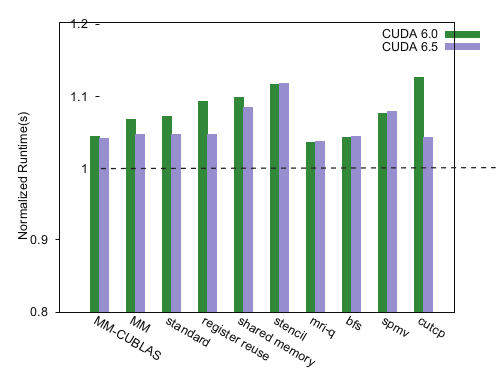
\includegraphics[width=0.9\linewidth]{unified_memory_benchmark_results}

They find that there are 10\% performance losses in average.
It is due to redundant memory transfers and page caching fault.
These losses are in some benchmarks considerably smaller under CUDA 6.5 than under CUDA 6.0.
The kernel running time in CUDA 6.5 does not improve.
It is the performance of launching and synchronizing what improves.
Interestingly, the TK1 uses the memory of CPU and GPU separately, even when it is physically one, resulting in uneeded copies.
It is also seen that pinned memory is used for Unified Memory.
It is revealed by the fact that copying times from host to device are much lower under Unified Memory.

Finally, five micro-benchmarks are created to look for the conditions causing the performance loss.
It is seen that memory is copied from host to device even if no kernel uses it.
Memory also gets copied back and forth even if it is only read by the GPU.
Only in the case that the CPU never reads or writes the data, are there no redundant memory transfers.

This same research group intends to analyze the performance under of Unified Memory in multi-GPU systems in the future.

\subsubsection{Unified Memory}
CUDA 4 introduced Unified Virtual Addressing.
UVA enabled pinning CPU memory to be accesible directly over PCIe without a memcpy.
This provided convenience but no performance.

Unified Memory was introduced in CUDA 6.
A single pointer referred to both CPU and GPU memory.
It worked through automatical data migration handled by software.
As described above, all managed memory touched by the CPU had to be synchronized.
Additionally, CPU and GPU could not access the same memory allocation simultaneously.
The address space was limited to the size of the GPU physical memory.

Now a single memory address space for CPU and GPU with 49-bit virtual addressing has been introduced.
Since current CPUs have up to 48-bit virtual addressing, this is enough to cover both spaces as a single virtual address space.
Now the memory limits of the GPU do not restrict the virtual space size.
Additionally, GP100 has hardware support for page faulting, which allows transparent access to data anywhere in the virtual address spaces.
This means there is no need for synchromization of all managed memory allocations.
The large address space allows direct addressing of very large datasets, much larger than the system memory.
Faulted pages are automatically migrated.
Mapping on access can sometimes be faster than migration (\textbf{TODO: When?})
CPUs can also fault and migrate memory from GPU.
CPU can even access data while a GPU kernel is running.
Coherency in this case could not be guaranteed in previous architectures.
Note that correct synchronization has to be taken care of as in any other parallel application.

Operating system support is being developed to enable GPUS to access memory allocated with the default OS allocator (such as malloc).

Aside from making GPU programming easier, this also allows easier use of C++ classes on GPU.
Any nested data can be automatically accessed thanks to the single virtual addres.

\subsubsection{Compute Preemption}
GP100 has preemption at instruction-level.
This is an improvement on block-level preemption of the Maxwell and Kepler architectures.
It allows interaction with long computing tasks, swapping contexts to GPU DRAM.
Otherwise, long running tasks can end up being killed by the OS or the CUDA driver.
Additionally, if a GPU is being used for display graphics and CUDA tasks, long running tasks can result in an unresponsive GUI.
This also makes interactive debugging work better.
Interactive debugging on Kepler and Maxwell required adding instrumentation during compilation to allow completion of thread blocks after an interrupt.
GP100 debugging is more robust and lightweight.


\subsection{Data transfer}
GPUDirect was introduced in Kepler allowed RDMA, lowering CPU overhead.
It enabled DMA, this means the CPU does not have to copy the data in its own memory.
It also enabled P2P data transfer between GPUs.
GPUDirect badnwidth is doubled in GP100.

Clusters of multi-GPU systems are being interconnected with InfiniBand(R) and 100Gb Ethernet.
The GPUs to CPUs ratio is increasing.
Fast cluster interconnections and this increasing ratio were causing PCIe to become a bottleneck.
That is why NVLink was introduced.
\subsubsection{NVLink}
Allows GPU-to-GPU data transfers.
It uses the new NVHS interconnect.
It is compatible with the GPU ISA, supporting shared memory multiprocessing.
Programs can execute directly on memory of another GPU with full capability.
Data is transmitted over a set of differential pairs with a bandwidth of 20Gb/sec each.
A total of 16 form a Link, with 8 pairs for each direction.
This gives a total bidirectional bandwidth of up to 40GB/sec
Since the GP100 supports up to 4 links, this allows up to 160GB/sec bidirectional data transfer.
PCIe Gen 3 x16, the largest in common use even though the standard is defined up to x32, provides a bandwidth of up to 31.75GB/s
A couple of GP100 cards can be connected with a bandwidth of up to more than 5x that of PCIe.

The NVLink controller is formed by a Pysical Layer, a Data Link Layer, and a Transaction Layer.
The package sizes range from 1 to 18 128-bit flits.
\textbf{TODO:}
The clock runs a t 1.25GHz.
It uses an embedded clock used at the received to capture data.
The Physical Layer takes care of deskewing across lanes, framing, scrambling/descrambling, polarity inversion and lane reversal.
% Polarity inversion and lane reversal allow for effective PCB routing.
The Data Link Layer is responsible for reliable transmission.
Packets are protected with a 25-bit CRC [\textbf{TODO}].
It is calculated over the current header and the previous payload.
It allows detection of up to 5 random bit errors or up to 25-bit bursts of errors on any lane.
Packets are stored in a replay buffer until the receiver acknowledges them.
If the transmitter times out waiting for acknowledgment, it starts retransmitting.

The Transaction Layer cares for synchromization, link flow control, virtual channels.
It can also aggregate multiple links together to provide higher communication bandwidth.

\subsection{TODOs}
\begin{itemize}
    \item Infiniband vs 100Gb Ethernet
\end{itemize}

% \begin{figure}[h]%
%  	\begin{center}%
%  		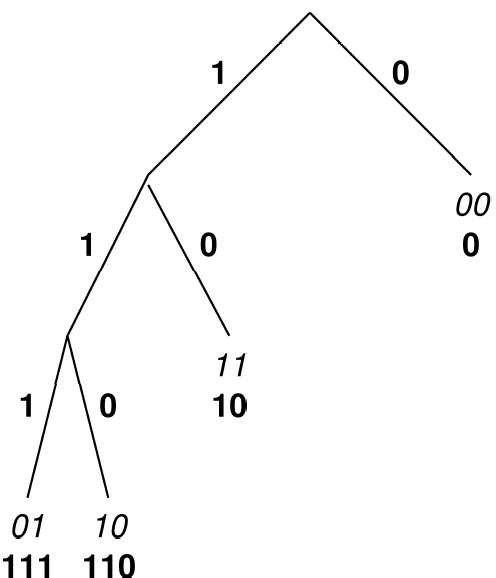
\includegraphics[scale=0.1]{figure1.png}%
%  		\caption{Baum}\label{fig:baum}%
%  	\end{center}%
% \end{figure}
%
% \begin{table}[h]%
%  	\begin{center}%
% 		\caption{Beispieltabelle}\label{tab:example}%
% 	 	\begin{tabular}{c|c}%
%  			Spalte1 & Spalte2\\
%  			\hline
%  			0 & 1\\
%  		\end{tabular}%
%  	\end{center}%
% \end{table}

% % can use a bibliography generated by BibTeX as a .bbl file
% % standard IEEE bibliography style from:
% % http://www.ctan.org/tex-archive/macros/latex/contrib/supported/IEEEtran/bibtex
% \bibliographystyle{IEEEtran}
% % argument is your BibTeX string definitions and bibliography database(s)
% \bibliography{IEEEabrv,references}
